\documentclass[preview]{standalone}

\usepackage{amsmath}
\usepackage{amssymb}
\usepackage{stellar}
\usepackage{definitions}

\begin{document}

\id{polynomials}
\genpage

\section{Polynomials}

% multiple indeterminates?
\begin{snippetdefinition}{polynomial-definition}{Polynomial}
    Let \((R, +, \cdot)\) be a \ring.
    A \textit{polynomial} over \(R\) is an expression of the form
    \[
        p(x)=\sum_{k=0}^n a_n x^n
    \]
    where \(a_n\in R\) and \(x\) is an indeterminate.
\end{snippetdefinition}

\plain{Every polynomial induces a corresponding function.}

\begin{snippetdefinition}{polynomial-degree-definition}{Polynomial degree}
    Given a \polynomial of the form
    \[
        p(x)=\sum_{k=0}^n a_n x^n
    \]
    the \textit{degree} of \(p(x)\), denoted \(\deg p(x)\),
    is the maximum index \(k\) such that \(a_k \neq 0\).
\end{snippetdefinition}

\begin{snippet}{null-polynomial-expl}
    The polynomial \(p(x)=0\) has no degree. However, sometimes it is
    convenient to say that it has degree \(-\infty\) or \(-1\).
\end{snippet}

\begin{snippetdefinition}{polynomial-root-multiplicity-definition}{Polynomial root multiplicity}
    Let \(P(x)\) be a \polynomial. Then, a root \(x_0\) of \(P(x)\)
    has \textit{multiplicity} \(m \in \naturalnumbers^\exceptzero\) if
    \(P(x)\) is divisible by \({(x-x_0)}^m\) but not \({(x-x_0)}^{m + 1}\).
\end{snippetdefinition}

\section{Polynomial division}

\begin{snippettheorem}{polynomial-division-theorem}{Polynomial division}
    Let \(f(x)\) and \(g(x)\) be two \polynomial[polynomials] over \(R\)
    where \(g(x)\neq0\).
    Then, there always exist two unique polynomials \(q(x)\) and \(r(x)\) over \(R\)
    such that \[ f(x)=g(x)q(x) + r(x) \]
    where \(r(x)=0\) or \(\polynomialdeg r(x) < \polynomialdeg g(x)\).
\end{snippettheorem}

\begin{snippetproof}{polynomial-division-proof}{polynomial-division-theorem}{Polynomial division}
    \textbf{Existence di \(q(x)\) and \(r(x)\):}
    Start with some initial value for \(q(x)\) and \(r(x)\)
    by letting \(q_0(x)=0\) and \(r_0=f(x)\) (so that the equation remains satisfied).
    
    If \(r_0(x)=0\) or \(\polynomialdeg r_0(x) < \polynomialdeg g(x)\) (i.e. the dividend is the null polynomials
    or its degree is less than the divisor), the process has already ended.
    Otherwise, we have the situation in which \(f(x) = a_0 + a_1x + \cdots + a_nx^n\)
    with \(a_n \neq 0\) and \(g(x)=b_0 + b_1x + \cdots + b_nx^m\) with \(a_m \neq 0\)
    where \(m \leq n\).
    
    The next step is to adjust the quotient, thus letting \[
        q_1(x)=q_0(x) + \frac{a_n}{b_m}x^{n-m}
        = \frac{a_n}{b_n}x^{n-m}
    \]
    and finding
    \begin{align*}
        r_1(x)=f(x)-q_1(x)g(x) &= a_0 + a_1 x \cdots a_n x^n - 
            \left(
            \frac{a_n}{b_m}x^{n-m}b_0 + \cdots + \frac{a_n}{b_m}x^{n-m}b_m x^m
        \right) \\
        &= a_nx^n - a_nx^n + \cdots
    \end{align*}
    
    And thus only remains terms of degree less than \(n\).
    Now \(r_1(x)=0\) or \(r_1(x)\) has degree less than \(r_0(x)=f(x)\) (the degree has diminuished).
    
    If \(r_1(x)=0\) or \(\polynomialdeg r_1(x) < \polynomialdeg g(x)\), the process has ended.
    Otherwise, if \(\polynomialdeg r_1(x) \geq \polynomialdeg g(x) = m\) the process is repeated.
    Eventually, remainders of smaller degrees will be found (or the null remainder),
    at which point the process has ended.
    The quotient and remainder are thus \(q_k(x)\) and \(r_k(x)\).
    \\
    \textbf{Uniqueness of \(q(x)\) and \(r(x)\):}
    Assume that \(f(x)=g(x)q(x) + r(x)=g(x)q'(x)+r'(x)\) with
    \(r(x)=0\) or \(\polynomialdeg r(x)<\deg g(x)\) and
    \(r'(x)=0\) or \(\polynomialdeg r'(x)<\polynomialdeg g(x)\).

    Starting from \(g(x)q(x)-g(x)q'(x)=r'(x)-r(x)\),
    we arrive at \(q(x)\left(q(x)-q'(x)\right) = r'(x)-r(x)\).

    For the proof we suppose that the quotient and remainder are not unique,
    so \(q(x)\neq q'(x)\) or \(q(x)-q'(x)\neq 0\),
    The first member should have a degree less than \(n\).
    The second member is null or it has degree less than \(n\).
    This is a contradiction, implying that quotient (and the remainder) are thus unique.
\end{snippetproof}

\begin{snippet}{polynomial-division-method-illustration}
    \begin{center}
        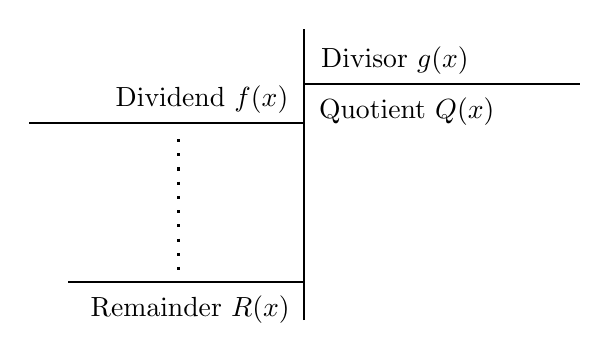
\begin{tikzpicture}
            %vline
            \draw[thick] (0,0) -- (0,3.7);
            %hlines
            \draw[thick] (0,3) -- (3.5,3);
            \draw[thick] (0,2.5) -- (-3.5,2.5);
            \draw[thick] (0,0.48) -- (-3,0.48);
            %dots
            \draw[line width=0.4mm, loosely dotted] (-1.6,2.3) -- (-1.6,0.6);
    
            %nodes
            \node at (1.15,3.3) {Divisor $g(x)$};
            \node at (-1.3,2.8) {Dividend $f(x)$};
            \node at (1.3,2.65) {Quotient $Q(x)$};
            \node at (-1.45,0.13) {Remainder $R(x)$};
        \end{tikzpicture}
    \end{center}
\end{snippet}

\section{Remainder theorem}

\begin{snippettheorem}{polynomial-remainder-theorem}{Remainder theorem}
    Let \(p(x)\) be a \polynomial and \(\alpha \in \complexnumbers\).
    The division of \(p(x)\) by \(x-\alpha\) has remainder \(p(\alpha)\)
    \[
        p(x) = q(x)(x-\alpha) + p(\alpha)
    \]
    for some \(q(x)\).
\end{snippettheorem}

\begin{snippetproof}{polynomial-remainder-proof}{polynomial-remainder-theorem}{Remainder theorem}
    By dividing \(p(\alpha)\) by \(x-\alpha\)
    we get
    \[
        p(x) = q(x)(x-\alpha) + r(x)
    \]
    for some \(q(x)\) and \(r(x)\),
    where either \(r(x)=0\) or \(\polynomialdeg r(x) < \polynomialdeg x-\alpha = 1\).
    So, \(r(x)\) is constant.
    We can now plug \(\alpha\) in and get
    \[ p(\alpha) = (\alpha - \alpha) q(\alpha) + r(\alpha) \]
    but \(r(\alpha)\) is constant, so we get
    \[ r(x) = p(\alpha) \]
\end{snippetproof}

\begin{snippetcorollary}{remainder-theorem-polynomial-root}{Root of polynomial}
    Given a \polynomial \(p(x)\), a value \(\alpha\)
    is a root of the polynomial \(p(\alpha) = 0\)
    \ifandonlyif \(p(x) = q(x)(x-\alpha)\) for some \polynomial \(q(x)\).
\end{snippetcorollary}

%\begin{snippetcorollary}{polynomial-divisibility-by-x-1}{Polynomial divisibility by \(x-1\)}
%    Let
%    \[ P(x) = \sum_{k=0}^n a_k x^k \]
%    be a \polynomial. Then, \(P(x)\)
%    is divisible by \(x-1\) if
%    \[ \sum_{k=0}^n a_k = 0 \]
%\end{snippetcorollary}

\section{Algebraic equations}

\begin{snippetdefinition}{algebraic-equation-definition}{Algebraic equation}
    An equation is said to be \textit{algebraic} if it has the form
    \[ f(x)=0\]
    where \(f(x)\) is a non-null \polynomial.
\end{snippetdefinition}


\begin{snippettheorem}{solutions-of-algebraic-equation-theorem}{Solutions of algebraic equations}
    Any \algebraicequation \(f(x)=0\) has at most \(n\) distinct solutions,
    where \(n=\polynomialdeg f(x)\).
\end{snippettheorem}

\begin{snippetproof}{solutions-of-algebraic-equation-proof}{solutions-of-algebraic-equation-theorem}{Solutions of algebraic equations}
    Let \(a_1\), \(a_2\), \(\cdots\), \(a_t\) be distinct solutions of \(f(x)=0\)
    where \(f(x)\) is non-null.
    We must show that \(t<n\).
    By the \snippetref[polynomial-remainder-theorem][remainder theorem] \(f(x)=(x-a_1)q_1(x)\) for some \polynomial \(q_1(x)\).\\
    The same goes for \(a_2\), \(a_3\), \(\cdots\).
    Substituting, we then get
    \(0=f(a_2)=(a_2-a_1)q_1(a_2)\).
    Since \(a_1 \neq a_2\), we have (by the cancellation principle)
    that \(q_1(a_2)=0\). By the \snippetref[polynomial-remainder-theorem][remainder theorem] \(q_1(x)=(x-a_2)q_2(x)\) for some \(q_2(x)\),
    and thus \(f(x) = (x-a_1)(x-a_2)q_2(x)\).
    By induction, we come to \(f(x)=(x-a_1)(x-a_2)\cdots(x-a_t)q_t(x)\)
    and by confronting the degrees we find that \(t \leq n\).
\end{snippetproof}

\end{document}